\section{Meal schedule}

The two figures in this section \cref{MealScheduleList} and \cref{MealScheduleBar} displays two design ideas for the meal schedule aspect of the program.

\begin{figure}[H]
	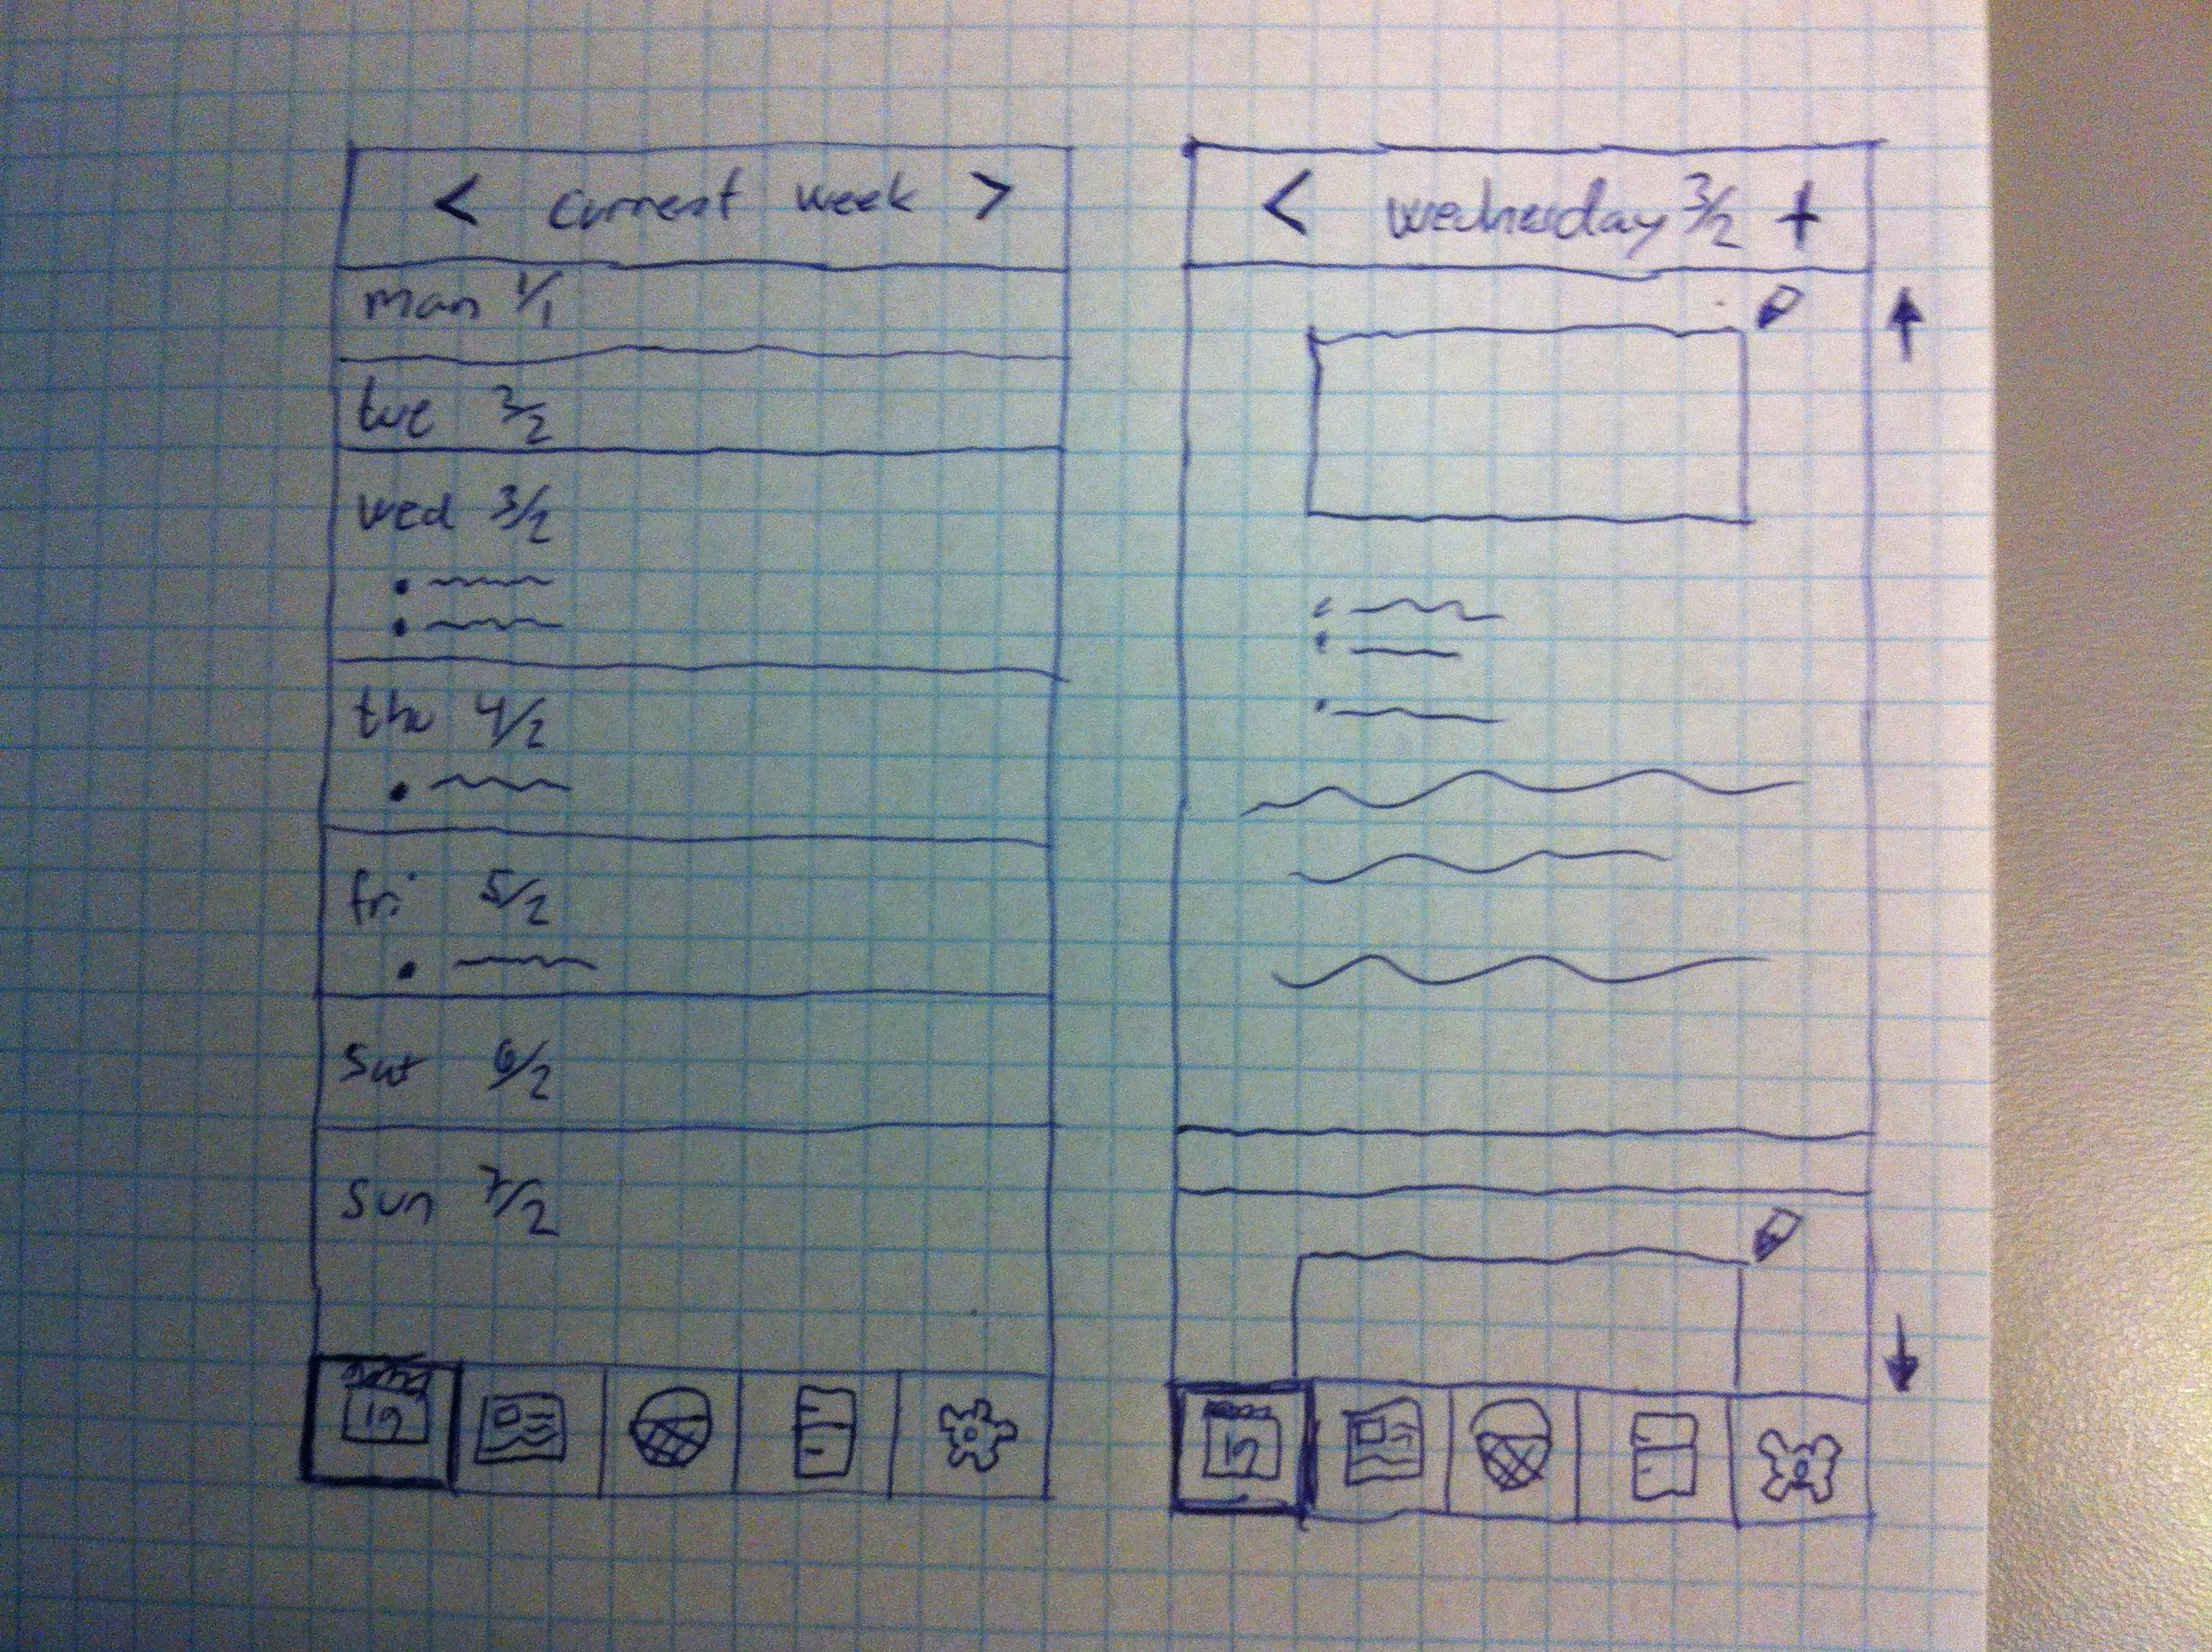
\includegraphics[width=0.8\textwidth]{Grafik/FoodPlanner/FinalMealScheduleSketch1}
	\caption{The right screen shows 7 days of a specific week and the left screen shows scheduled meals on a specific day.}
	\label{MealScheduleList}
\end{figure}

Beginning with the screen to the left on \cref{MealScheduleList} there are three areas of concern. In the middle of the screen there is a list overview of 7 days. Each day shows the name, date, ingredients that the user has of scheduled meals on a specific day. If there are many meals scheduled the list will expand to outside of the screen view. The user can scroll to view all days and press a specific day to view details about it. This method of display gives the user an easy and informative view of the week days. The top bar is used to navigate between weeks. The left screen on \cref{MealScheduleList} displays the screen for a specific day. The navigation bar on the bottom is unchanged. On the middle there are an overview of all the planned recipes which the user can scroll through. On each of the recipe there is a icon for the user to change a specific meal. The meals will display information such as ingredients, title, number of participant. The top bar has a button to add meals to the specific day and it also shows what day it is and an arrow for the user to navigate back to the week overview.  

\begin{figure}[H]
	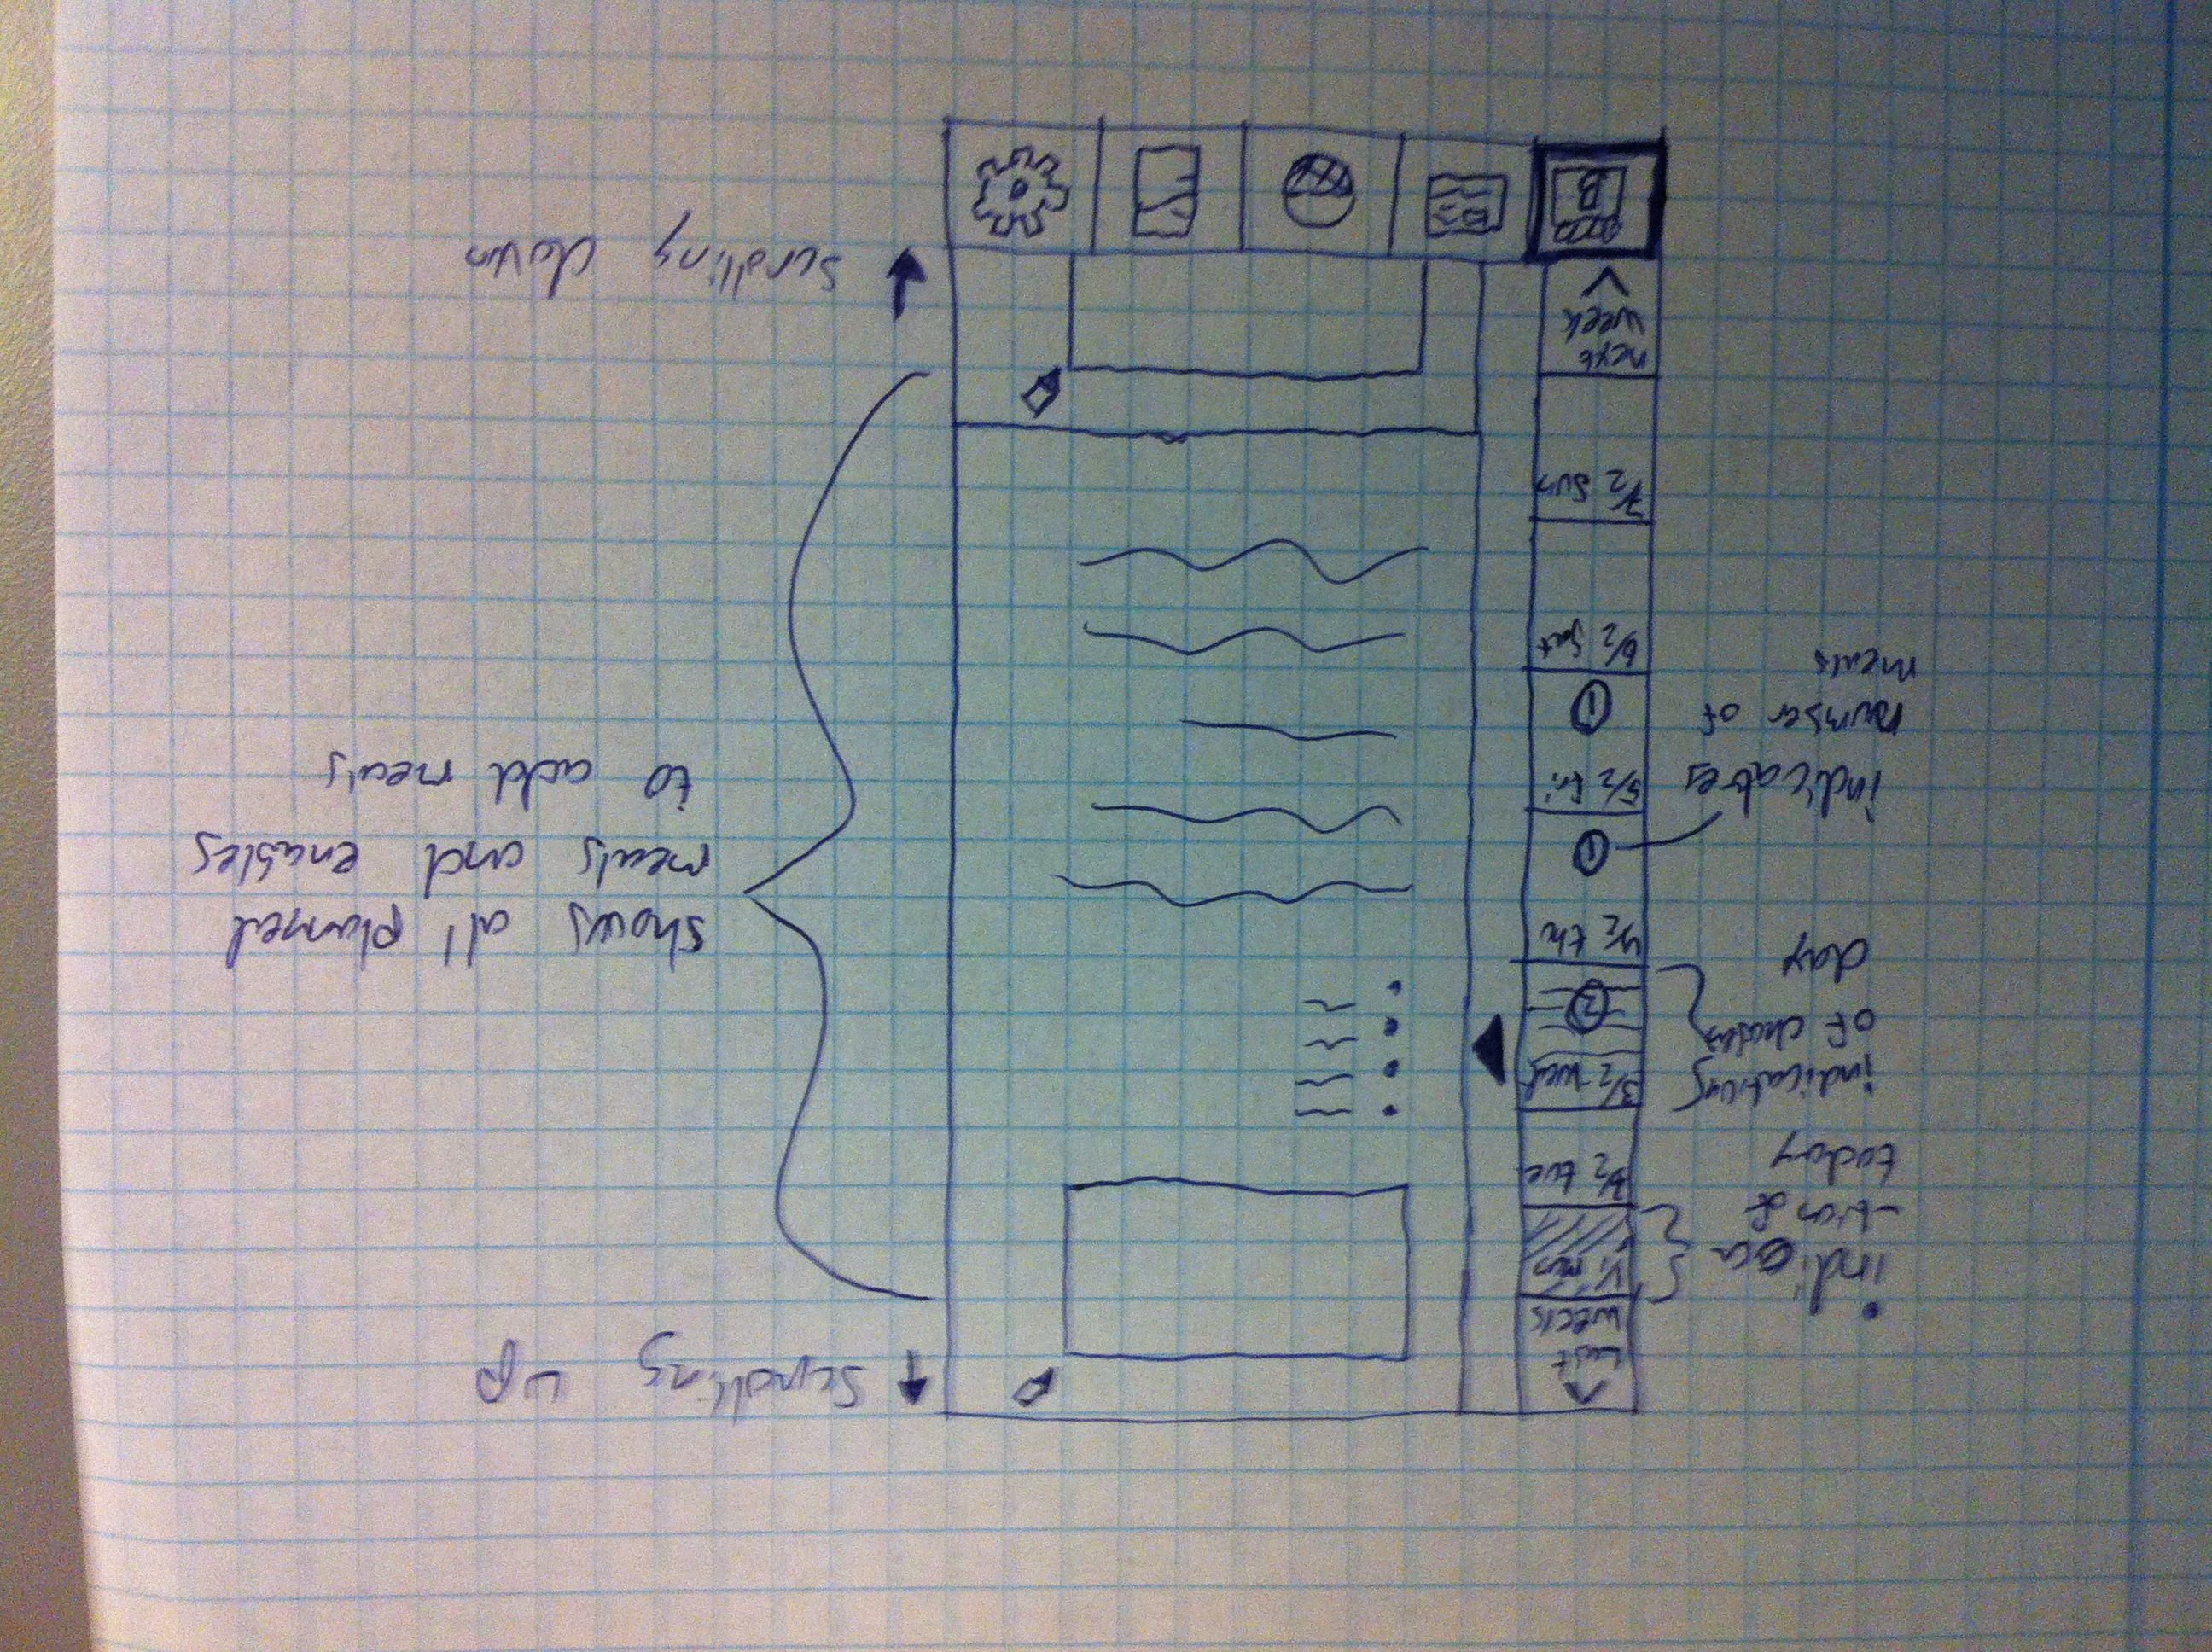
\includegraphics[width=0.8\textwidth]{Grafik/FoodPlanner/FinalMealScheduleSketch2}
	\caption{This sketch merges both of the screens above into one screen with the weeks on the left bar and the scheduled meals as a list on the right side of the screen.}
	\label{MealScheduleBar}
\end{figure}

On \cref{MealScheduleList} there a displayed a different approach to the design of the meal schedule. This screen has a weekly overview on the left bar. At the top and bottom of this bar there are buttons to navigate between weeks. Each day on this bar has a title, date and a indication of the number of scheduled meals. There are also an indication of the current day and the day that has been selected. On  the left side of the screen there is an overview of the scheduled meals just as the method used on the right screen on \cref{MealScheduleList}. 

